\documentclass[]{article}
\usepackage{lmodern}
\usepackage{amssymb,amsmath}
\usepackage{ifxetex,ifluatex}
\usepackage{fixltx2e} % provides \textsubscript
\ifnum 0\ifxetex 1\fi\ifluatex 1\fi=0 % if pdftex
  \usepackage[T1]{fontenc}
  \usepackage[utf8]{inputenc}
\else % if luatex or xelatex
  \ifxetex
    \usepackage{mathspec}
  \else
    \usepackage{fontspec}
  \fi
  \defaultfontfeatures{Ligatures=TeX,Scale=MatchLowercase}
\fi
% use upquote if available, for straight quotes in verbatim environments
\IfFileExists{upquote.sty}{\usepackage{upquote}}{}
% use microtype if available
\IfFileExists{microtype.sty}{%
\usepackage{microtype}
\UseMicrotypeSet[protrusion]{basicmath} % disable protrusion for tt fonts
}{}
\usepackage[margin=1in]{geometry}
\usepackage{hyperref}
\hypersetup{unicode=true,
            pdfborder={0 0 0},
            breaklinks=true}
\urlstyle{same}  % don't use monospace font for urls
\usepackage{color}
\usepackage{fancyvrb}
\newcommand{\VerbBar}{|}
\newcommand{\VERB}{\Verb[commandchars=\\\{\}]}
\DefineVerbatimEnvironment{Highlighting}{Verbatim}{commandchars=\\\{\}}
% Add ',fontsize=\small' for more characters per line
\usepackage{framed}
\definecolor{shadecolor}{RGB}{248,248,248}
\newenvironment{Shaded}{\begin{snugshade}}{\end{snugshade}}
\newcommand{\KeywordTok}[1]{\textcolor[rgb]{0.13,0.29,0.53}{\textbf{#1}}}
\newcommand{\DataTypeTok}[1]{\textcolor[rgb]{0.13,0.29,0.53}{#1}}
\newcommand{\DecValTok}[1]{\textcolor[rgb]{0.00,0.00,0.81}{#1}}
\newcommand{\BaseNTok}[1]{\textcolor[rgb]{0.00,0.00,0.81}{#1}}
\newcommand{\FloatTok}[1]{\textcolor[rgb]{0.00,0.00,0.81}{#1}}
\newcommand{\ConstantTok}[1]{\textcolor[rgb]{0.00,0.00,0.00}{#1}}
\newcommand{\CharTok}[1]{\textcolor[rgb]{0.31,0.60,0.02}{#1}}
\newcommand{\SpecialCharTok}[1]{\textcolor[rgb]{0.00,0.00,0.00}{#1}}
\newcommand{\StringTok}[1]{\textcolor[rgb]{0.31,0.60,0.02}{#1}}
\newcommand{\VerbatimStringTok}[1]{\textcolor[rgb]{0.31,0.60,0.02}{#1}}
\newcommand{\SpecialStringTok}[1]{\textcolor[rgb]{0.31,0.60,0.02}{#1}}
\newcommand{\ImportTok}[1]{#1}
\newcommand{\CommentTok}[1]{\textcolor[rgb]{0.56,0.35,0.01}{\textit{#1}}}
\newcommand{\DocumentationTok}[1]{\textcolor[rgb]{0.56,0.35,0.01}{\textbf{\textit{#1}}}}
\newcommand{\AnnotationTok}[1]{\textcolor[rgb]{0.56,0.35,0.01}{\textbf{\textit{#1}}}}
\newcommand{\CommentVarTok}[1]{\textcolor[rgb]{0.56,0.35,0.01}{\textbf{\textit{#1}}}}
\newcommand{\OtherTok}[1]{\textcolor[rgb]{0.56,0.35,0.01}{#1}}
\newcommand{\FunctionTok}[1]{\textcolor[rgb]{0.00,0.00,0.00}{#1}}
\newcommand{\VariableTok}[1]{\textcolor[rgb]{0.00,0.00,0.00}{#1}}
\newcommand{\ControlFlowTok}[1]{\textcolor[rgb]{0.13,0.29,0.53}{\textbf{#1}}}
\newcommand{\OperatorTok}[1]{\textcolor[rgb]{0.81,0.36,0.00}{\textbf{#1}}}
\newcommand{\BuiltInTok}[1]{#1}
\newcommand{\ExtensionTok}[1]{#1}
\newcommand{\PreprocessorTok}[1]{\textcolor[rgb]{0.56,0.35,0.01}{\textit{#1}}}
\newcommand{\AttributeTok}[1]{\textcolor[rgb]{0.77,0.63,0.00}{#1}}
\newcommand{\RegionMarkerTok}[1]{#1}
\newcommand{\InformationTok}[1]{\textcolor[rgb]{0.56,0.35,0.01}{\textbf{\textit{#1}}}}
\newcommand{\WarningTok}[1]{\textcolor[rgb]{0.56,0.35,0.01}{\textbf{\textit{#1}}}}
\newcommand{\AlertTok}[1]{\textcolor[rgb]{0.94,0.16,0.16}{#1}}
\newcommand{\ErrorTok}[1]{\textcolor[rgb]{0.64,0.00,0.00}{\textbf{#1}}}
\newcommand{\NormalTok}[1]{#1}
\usepackage{longtable,booktabs}
\usepackage{graphicx,grffile}
\makeatletter
\def\maxwidth{\ifdim\Gin@nat@width>\linewidth\linewidth\else\Gin@nat@width\fi}
\def\maxheight{\ifdim\Gin@nat@height>\textheight\textheight\else\Gin@nat@height\fi}
\makeatother
% Scale images if necessary, so that they will not overflow the page
% margins by default, and it is still possible to overwrite the defaults
% using explicit options in \includegraphics[width, height, ...]{}
\setkeys{Gin}{width=\maxwidth,height=\maxheight,keepaspectratio}
\IfFileExists{parskip.sty}{%
\usepackage{parskip}
}{% else
\setlength{\parindent}{0pt}
\setlength{\parskip}{6pt plus 2pt minus 1pt}
}
\setlength{\emergencystretch}{3em}  % prevent overfull lines
\providecommand{\tightlist}{%
  \setlength{\itemsep}{0pt}\setlength{\parskip}{0pt}}
\setcounter{secnumdepth}{0}
% Redefines (sub)paragraphs to behave more like sections
\ifx\paragraph\undefined\else
\let\oldparagraph\paragraph
\renewcommand{\paragraph}[1]{\oldparagraph{#1}\mbox{}}
\fi
\ifx\subparagraph\undefined\else
\let\oldsubparagraph\subparagraph
\renewcommand{\subparagraph}[1]{\oldsubparagraph{#1}\mbox{}}
\fi

%%% Use protect on footnotes to avoid problems with footnotes in titles
\let\rmarkdownfootnote\footnote%
\def\footnote{\protect\rmarkdownfootnote}

%%% Change title format to be more compact
\usepackage{titling}

% Create subtitle command for use in maketitle
\newcommand{\subtitle}[1]{
  \posttitle{
    \begin{center}\large#1\end{center}
    }
}

\setlength{\droptitle}{-2em}

  \title{}
    \pretitle{\vspace{\droptitle}}
  \posttitle{}
    \author{}
    \preauthor{}\postauthor{}
    \date{}
    \predate{}\postdate{}
  

\begin{document}

\section{Cover Sheet}\label{cover-sheet}

By including this statement, we, all the students listed in the table
below, declare that:

\begin{itemize}
\item
  We hold a copy of this assignment if the original is lost or damaged.
\item
  We hereby certify that no part of this assignment has been copied from
  any other student's work or from any other source except where due
  acknowledgement is made in the assignment.
\item
  No part of the assignment has been written for us by any other person
  except where collaboration has been authorised by the unit
  coordinator.
\item
  We are aware that this work may be reproduced and submitted to
  plagiarism detection software programs for the purpose of detecting
  possible plagiarism; this software may retain a copy on its database
  for future plagiarism checking.
\item
  We hereby certify that no part of this assignment or product has been
  submitted by any of us in another (previous or current) assessment,
  except where appropriately referenced, and with prior permission from
  the unit coordinator for this unit.
\item
  We hereby certify that we have read and understand what the University
  considers to be academic misconduct, and that we are aware of the
  penalties that may be imposed for academic misconduct.
\end{itemize}

\begin{longtable}[]{@{}lll@{}}
\toprule
Name & Student Number & Contribution (\%)\tabularnewline
\midrule
\endhead
Rachel Hardie & 18820821 & 25\%\tabularnewline
Dylan Wang & 18998014 & 25\%\tabularnewline
Dylan Yoo & 18640377 & 25\%\tabularnewline
Sreenath Ramachandran & 18878716 & 25\%\tabularnewline
\bottomrule
\end{longtable}

\begin{Shaded}
\begin{Highlighting}[]
\KeywordTok{library}\NormalTok{(}\StringTok{"tm"}\NormalTok{)}
\KeywordTok{library}\NormalTok{(}\StringTok{"rtweet"}\NormalTok{)}
\KeywordTok{library}\NormalTok{(}\StringTok{"twitteR"}\NormalTok{)}
\KeywordTok{library}\NormalTok{(}\StringTok{"igraph"}\NormalTok{)}
\KeywordTok{library}\NormalTok{(}\StringTok{"knitr"}\NormalTok{)}
\NormalTok{tweets=}\KeywordTok{read.csv}\NormalTok{(}\StringTok{"SWAProject.csv"}\NormalTok{)}
\end{Highlighting}
\end{Shaded}

We then constructed a document-term matrix using TFIDF weighting to
describe the frequency of terms in the tweets we had collected.

\begin{Shaded}
\begin{Highlighting}[]
\NormalTok{corpus=}\KeywordTok{Corpus}\NormalTok{(}\KeywordTok{VectorSource}\NormalTok{(tweets}\OperatorTok{$}\NormalTok{text))}
\NormalTok{corpus =}\StringTok{ }\KeywordTok{tm_map}\NormalTok{(corpus, }\ControlFlowTok{function}\NormalTok{(x) }\KeywordTok{iconv}\NormalTok{(x, }\DataTypeTok{to =} \StringTok{'UTF8'}\NormalTok{, }\DataTypeTok{sub =} \StringTok{'byte'}\NormalTok{))}
\NormalTok{corpus =}\StringTok{ }\KeywordTok{tm_map}\NormalTok{(corpus, }\ControlFlowTok{function}\NormalTok{(x) }\KeywordTok{iconv}\NormalTok{(x, }\DataTypeTok{to =} \StringTok{'ASCII'}\NormalTok{, }\DataTypeTok{sub =} \StringTok{' '}\NormalTok{))}
\NormalTok{corpus =}\StringTok{ }\KeywordTok{tm_map}\NormalTok{(corpus,removeNumbers)}
\NormalTok{corpus =}\StringTok{ }\KeywordTok{tm_map}\NormalTok{(corpus, removeWords,}\KeywordTok{c}\NormalTok{(}\KeywordTok{stopwords}\NormalTok{(),}\StringTok{"J.K. Rowling"}\NormalTok{,}\StringTok{"https"}\NormalTok{, }\StringTok{"t.co"}\NormalTok{))}
\NormalTok{corpus =}\StringTok{ }\KeywordTok{tm_map}\NormalTok{(corpus,removePunctuation)}
\NormalTok{corpus =}\StringTok{ }\KeywordTok{tm_map}\NormalTok{(corpus,stripWhitespace)}
\NormalTok{corpus =}\StringTok{ }\KeywordTok{tm_map}\NormalTok{(corpus, tolower)}
\NormalTok{corpus =}\StringTok{ }\KeywordTok{tm_map}\NormalTok{(corpus, stemDocument)}
\NormalTok{corpus =}\StringTok{ }\KeywordTok{tm_map}\NormalTok{(corpus, removeWords,}\KeywordTok{c}\NormalTok{(}\KeywordTok{stopwords}\NormalTok{(),}\StringTok{"jk"}\NormalTok{,}\StringTok{"https"}\NormalTok{, }\StringTok{"t.co"}\NormalTok{,}\StringTok{"rowl"}\NormalTok{,}\StringTok{"jkrowl"}\NormalTok{,}
                                      \StringTok{"will"}\NormalTok{,}\StringTok{"like"}\NormalTok{,}\StringTok{"just"}\NormalTok{,}\StringTok{"doe"}\NormalTok{,}\StringTok{"far"}\NormalTok{,}\StringTok{"quot"}\NormalTok{,}\StringTok{"look"}\NormalTok{,}
                                      \StringTok{"take"}\NormalTok{,}\StringTok{"make"}\NormalTok{,}\StringTok{"jaqkcpmtg"}\NormalTok{,}\StringTok{"ygorfremo"}\NormalTok{,}\StringTok{"ask"}\NormalTok{,}\StringTok{"peopl"}\NormalTok{,}
                                      \StringTok{"next"}\NormalTok{,}\StringTok{"twitter"}\NormalTok{,}\StringTok{"peopl"}\NormalTok{,}\StringTok{"new"}\NormalTok{,}\StringTok{"write"}\NormalTok{,}\StringTok{"charact"}\NormalTok{,}\StringTok{"got"}\NormalTok{,}
                                      \StringTok{"ohhgmljqrm"}\NormalTok{,}\StringTok{"say"}\NormalTok{,}\StringTok{"defend"}\NormalTok{,}\StringTok{"respond"}\NormalTok{, }\StringTok{"vrmgsnrsa"}\NormalTok{,}
                                      \StringTok{"bbepgeik"}\NormalTok{,}\StringTok{"nkuwxgsn"}\NormalTok{,}\StringTok{"novrijqr"}\NormalTok{,}\StringTok{"nlrbgguhxt"}\NormalTok{))}
\NormalTok{dtm =}\StringTok{ }\KeywordTok{DocumentTermMatrix}\NormalTok{(corpus)}
\NormalTok{tweet.wdtm =}\StringTok{ }\KeywordTok{weightTfIdf}\NormalTok{(dtm)}
\NormalTok{tweet.matrix =}\StringTok{ }\KeywordTok{as.matrix}\NormalTok{(tweet.wdtm)}
\end{Highlighting}
\end{Shaded}

\subsection{Finding the similarity
index}\label{finding-the-similarity-index}

To find the cosine similarity matrix we first find the normalised tweet
matrix.

\begin{Shaded}
\begin{Highlighting}[]
\CommentTok{#Find similarity matrix}
\NormalTok{S=tweet.matrix}\OperatorTok\KeywordTok{t}\NormalTok{(tweet.matrix)}
\CommentTok{#to find the cosine similarity matrix we need  the normalised tweet matrix.}
\NormalTok{norm.tweet.matrix =}\StringTok{ }\KeywordTok{diag}\NormalTok{(}\DecValTok{1}\OperatorTok{/}\KeywordTok{sqrt}\NormalTok{(}\KeywordTok{rowSums}\NormalTok{(tweet.matrix}\OperatorTok{^}\DecValTok{2}\NormalTok{))) }\OperatorTok\StringTok{ }\NormalTok{tweet.matrix}
\CommentTok{#cosine similarity}
\NormalTok{CS=norm.tweet.matrix}\OperatorTok\KeywordTok{t}\NormalTok{(norm.tweet.matrix)}

\KeywordTok{head}\NormalTok{(S)[}\DecValTok{1}\OperatorTok{:}\DecValTok{20}\NormalTok{]}
\end{Highlighting}
\end{Shaded}

\begin{verbatim}
##  [1] 2.78426986 0.00000000 0.00000000 0.00000000 0.00000000 0.23041424
##  [7] 0.00000000 0.49056435 0.05247791 0.10696634 0.49056435 0.00000000
## [13] 0.00000000 0.05247791 1.30694847 0.00000000 0.05247791 0.00000000
## [19] 0.00000000 0.10696634
\end{verbatim}

\begin{Shaded}
\begin{Highlighting}[]
\KeywordTok{head}\NormalTok{(CS)[}\DecValTok{1}\OperatorTok{:}\DecValTok{20}\NormalTok{]}
\end{Highlighting}
\end{Shaded}

\begin{verbatim}
##  [1] 1.00000000 0.00000000 0.00000000 0.00000000 0.00000000 0.07619747
##  [7] 0.00000000 1.00000000 0.06553893 0.06550168 1.00000000 0.00000000
## [13] 0.00000000 0.06553893 1.00000000 0.00000000 0.06553893 0.00000000
## [19] 0.00000000 0.06550168
\end{verbatim}

\subsection{Difference between Cosine similarity and
S}\label{difference-between-cosine-similarity-and-s}

Cosine similarity gives the angle between the documents. The similarity
matrix is more like the magnitude of the difference between the
documents whereas the cosine similarity matrix gives the
direction.Cosine similarity of the documents will be between 0 and 1.
\#\#8.4.2 As the histogram of retweet count is exponenetial we take
logarithm of retweet counts we take the log of retweet count+1 so as to
eliminate log 0 from the data

\begin{Shaded}
\begin{Highlighting}[]
\CommentTok{#8.4.2}
\NormalTok{retweetCount=tweets}\OperatorTok{$}\NormalTok{retweet_count}

\KeywordTok{hist}\NormalTok{(retweetCount)}
\end{Highlighting}
\end{Shaded}

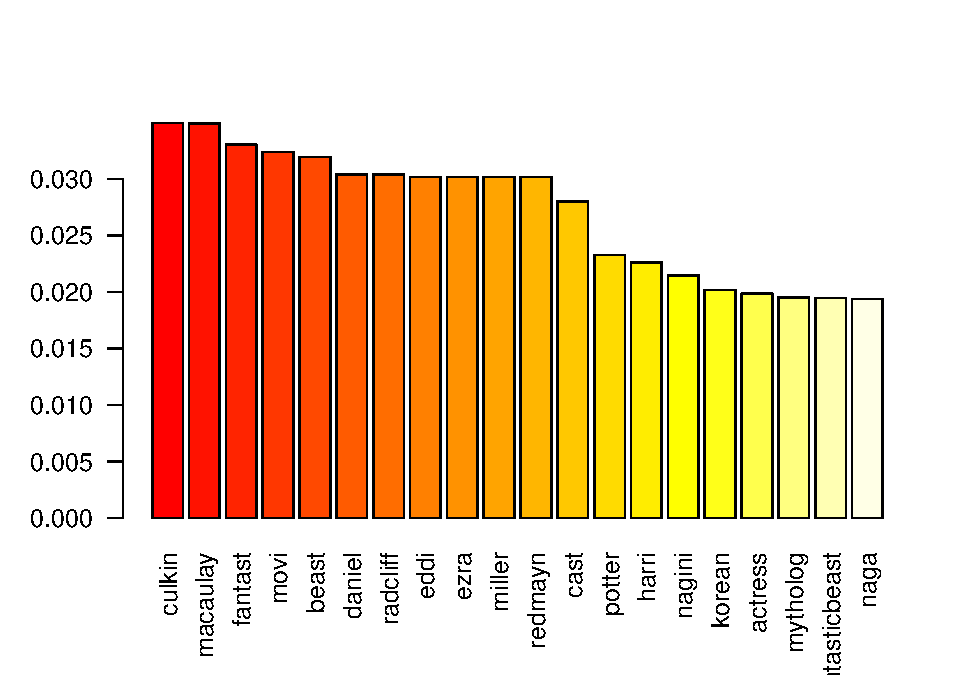
\includegraphics{PartB_files/figure-latex/unnamed-chunk-4-1.pdf}

\begin{Shaded}
\begin{Highlighting}[]
\KeywordTok{hist}\NormalTok{(}\KeywordTok{log}\NormalTok{(retweetCount}\OperatorTok{+}\DecValTok{1}\NormalTok{))}
\end{Highlighting}
\end{Shaded}

\includegraphics{PartB_files/figure-latex/unnamed-chunk-4-2.pdf}

\subsection{8.4.3}\label{section}

To make the graph simpler we are taking the top 20 retweeted tweets.

\begin{Shaded}
\begin{Highlighting}[]
\NormalTok{graph=}\KeywordTok{graph.adjacency}\NormalTok{(S,}\DataTypeTok{weighted =} \OtherTok{TRUE}\NormalTok{)}
\KeywordTok{plot}\NormalTok{(}\KeywordTok{simplify}\NormalTok{(graph),}\DataTypeTok{layout =}\NormalTok{ layout.drl,}\DataTypeTok{vertex.size=}\KeywordTok{log}\NormalTok{(retweetCount}\OperatorTok{+}\DecValTok{1}\NormalTok{))}
\end{Highlighting}
\end{Shaded}

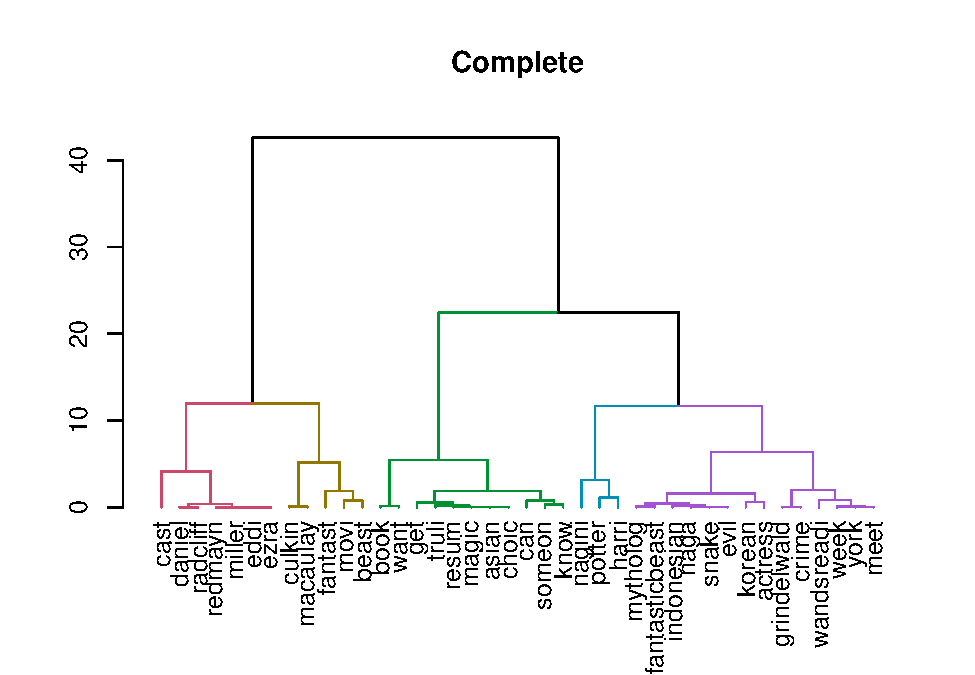
\includegraphics{PartB_files/figure-latex/unnamed-chunk-5-1.pdf}

\begin{Shaded}
\begin{Highlighting}[]
\CommentTok{# to make the graph simpler we are taking the top 20 retweeted tweets.}
\NormalTok{id=}\KeywordTok{order}\NormalTok{(}\KeywordTok{log}\NormalTok{(retweetCount}\OperatorTok{+}\DecValTok{1}\NormalTok{),}\DataTypeTok{decreasing =} \OtherTok{TRUE}\NormalTok{)[}\DecValTok{1}\OperatorTok{:}\DecValTok{20}\NormalTok{]}
\NormalTok{tweets.imp=tweets[id,]}
\NormalTok{retweetCount.imp=tweets.imp}\OperatorTok{$}\NormalTok{retweet_count}
\CommentTok{#retweetCount.imp}
\NormalTok{tweet.imp=tweet.matrix[id,]}
\NormalTok{s.imp=tweet.imp}\OperatorTok\KeywordTok{t}\NormalTok{(tweet.imp)}
\KeywordTok{set.seed}\NormalTok{(}\DecValTok{1500}\NormalTok{)}
\NormalTok{graph1=}\KeywordTok{graph.adjacency}\NormalTok{(s.imp,}\DataTypeTok{weighted =} \OtherTok{TRUE}\NormalTok{)}
\KeywordTok{plot}\NormalTok{(}\KeywordTok{simplify}\NormalTok{(graph1),}\DataTypeTok{layout=}\NormalTok{layout.auto,}
     \DataTypeTok{vertex.size=}\KeywordTok{log}\NormalTok{(retweetCount.imp}\OperatorTok{+}\DecValTok{1}\NormalTok{),}
     \DataTypeTok{edge.arrow.size=}\FloatTok{0.1}\NormalTok{,}\DataTypeTok{vertex.label.size=}\NormalTok{.}\DecValTok{5}\NormalTok{,}\DataTypeTok{vertex.label.color=}\StringTok{"black"}\NormalTok{)}
\end{Highlighting}
\end{Shaded}

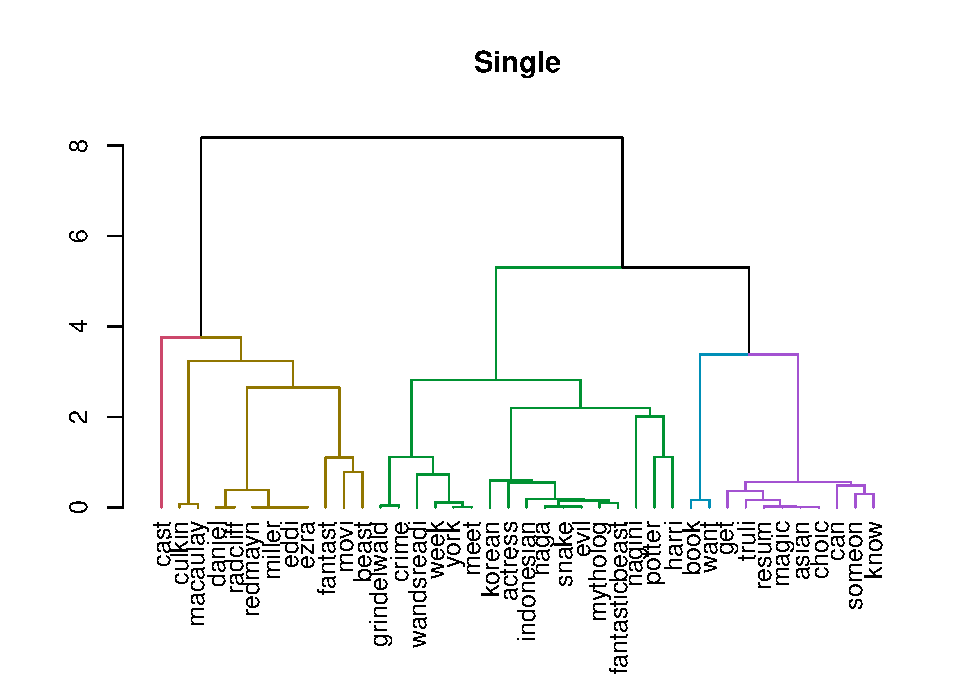
\includegraphics{PartB_files/figure-latex/unnamed-chunk-5-2.pdf}

\subsubsection{Results}\label{results}

Connected tweets mostly are the same tweets retweeted by different
users.

\subsection{8.5.1}\label{section-1}

\subsubsection{Degree centrality}\label{degree-centrality}

\begin{Shaded}
\begin{Highlighting}[]
\NormalTok{degCentrality=}\KeywordTok{degree}\NormalTok{(graph)}
\NormalTok{topTweetsDegree=}\KeywordTok{order}\NormalTok{(}\KeywordTok{degree}\NormalTok{(graph),}\DataTypeTok{decreasing =} \OtherTok{TRUE}\NormalTok{)[}\DecValTok{1}\OperatorTok{:}\DecValTok{10}\NormalTok{]}
\NormalTok{tweets}\OperatorTok{$}\NormalTok{text[topTweetsDegree]}
\end{Highlighting}
\end{Shaded}

\begin{verbatim}
##  [1] Macaulay Culkin tweets at J.K. Rowling asking for a job - https://t.co/BYCO6Q5Rjd \n\nMacaulay Culkin wants to be part of J.K. Rowlingâ\200\230s Harry Potter universe.\nAfter receiving some backlash for casting an Asian actress as a villainâ\200\231s slave in the upcoming â\200œFantastic Beast...                                                           
##  [2] Harry Potter fans really want Macaulay Culkin to get a part in Fantastic Beasts after his tweet to J.K. Rowling\nhttps://t.co/MZnaUpyggm https://t.co/CrYlJKjx26                                                                                                                                                                                      
##  [3] #1 (and only) reason I will never watch Harry Potter movies (including Fantastic Beasts) or read any of the books? J.K. Rowling.                                                                                                                                                                                                                      
##  [4] Elijah, I also see that Macaulay has talked to J.K. Rowling about being cast in the Fantastic Beast movie.. I'm glad to know he's back into the movies.. Feel free to write me messages on Twitter or E-Mail me at some time if you want to!!!!                                                                                                       
##  [5] @hermioneswife @jahuraaa @piccolosturban @luciusobsessed Yikes. Tbh does J.K. Rowling even get to chose the casting 100% just from the Harry Potter series alone there werenâ\200\231t poc at all. Or the few poc described in the book werenâ\200\231t in the film or mentioned in the film                                                                      
##  [6] J.K. Rowling confirms massive fan conspiracy in 'Harry Potter' universe The final trailer for the highly anticipated second installment of the "Fantastic Beasts" franchise, "The Crimes of... https://t.co/igWMjjgREQ                                                                                                                                
##  [7] I don't really have an issue with Nagini being cast as a Korean woman. No problem there.\n\nI do, however, have a problem with J.K. Rowling pulling random out of her ass about the Wizarding World.\n\nI get it: she wrote it, she can do what she wants. But it still comes across as lazy                                                          
##  [8] I've read fantastic beasts and where to find me but there isn't a book about the Crimes of Grindelwald, that I know. \n\nBut I know F.B is an extention of the wizarding world that J.K Rowling recently started. https://t.co/yKKNjU5fKj                                                                                                             
##  [9] Macaulay Culkin sent his CV to J.K. Rowling for a part in Fantastic Beasts - now people really want him to be cast - https://t.co/sNCq6qT5AS https://t.co/3hlb8ulVbk                                                                                                                                                                                  
## [10] J K Rowling being J K Rowling. Seven books and not a single peep. In deathly hallows, Nagini is an old woman ready to jump harry. But Maledictus turn into beasts PERMANENTLY <U+0001F926><U+0001F3FE><U+200D><U+2642><U+FE0F><U+0001F926><U+0001F3FE><U+200D><U+2642><U+FE0F><U+0001F926><U+0001F3FE><U+200D><U+2642><U+FE0F> https://t.co/l4Um3gIHVV
## 412 Levels: 'A racist, misogynist disaster': J.K. Rowling responds as fans slam Fantastic Beasts casting\nhttps://t.co/u1aQMhhkDV ...
\end{verbatim}

\subsubsection{Closeness centrality}\label{closeness-centrality}

\begin{Shaded}
\begin{Highlighting}[]
\NormalTok{closenessCentrality=}\KeywordTok{closeness}\NormalTok{(graph)}
\end{Highlighting}
\end{Shaded}

\begin{verbatim}
## Warning in closeness(graph): At centrality.c:2617 :closeness centrality is
## not well-defined for disconnected graphs
\end{verbatim}

\begin{Shaded}
\begin{Highlighting}[]
\NormalTok{topTweetsCloseness=}\KeywordTok{order}\NormalTok{(}\KeywordTok{closeness}\NormalTok{(graph),}\DataTypeTok{decreasing =} \OtherTok{TRUE}\NormalTok{)[}\DecValTok{1}\OperatorTok{:}\DecValTok{10}\NormalTok{]}
\end{Highlighting}
\end{Shaded}

\begin{verbatim}
## Warning in closeness(graph): At centrality.c:2617 :closeness centrality is
## not well-defined for disconnected graphs
\end{verbatim}

\begin{Shaded}
\begin{Highlighting}[]
\NormalTok{tweets}\OperatorTok{$}\NormalTok{text[topTweetsCloseness]}
\end{Highlighting}
\end{Shaded}

\begin{verbatim}
##  [1] Me in 2016: "Oh boy, more movies set in the Harry Potter universe, written by J.K. Rowling herself! This should be fascinati--"\n\n2018: "Abusey McSparrowHatter is our bad guy and Nagini was a Korean lady the whole time."\n\nMe: https://t.co/mXO3IXzDSM                                          
##  [2] Me in 2016: "Oh boy, more movies set in the Harry Potter universe, written by J.K. Rowling herself! This should be fascinati--"\n\n2018: "Abusey McSparrowHatter is our bad guy and Nagini was a Korean lady the whole time."\n\nMe: https://t.co/mXO3IXzDSM                                          
##  [3] Me in 2016: "Oh boy, more movies set in the Harry Potter universe, written by J.K. Rowling herself! This should be fascinati--"\n\n2018: "Abusey McSparrowHatter is our bad guy and Nagini was a Korean lady the whole time."\n\nMe: https://t.co/mXO3IXzDSM                                          
##  [4] Me in 2016: "Oh boy, more movies set in the Harry Potter universe, written by J.K. Rowling herself! This should be fascinati--"\n\n2018: "Abusey McSparrowHatter is our bad guy and Nagini was a Korean lady the whole time."\n\nMe: https://t.co/mXO3IXzDSM                                          
##  [5] Me in 2016: "Oh boy, more movies set in the Harry Potter universe, written by J.K. Rowling herself! This should be fascinati--"\n\n2018: "Abusey McSparrowHatter is our bad guy and Nagini was a Korean lady the whole time."\n\nMe: https://t.co/mXO3IXzDSM                                          
##  [6] Me in 2016: "Oh boy, more movies set in the Harry Potter universe, written by J.K. Rowling herself! This should be fascinati--"\n\n2018: "Abusey McSparrowHatter is our bad guy and Nagini was a Korean lady the whole time."\n\nMe: https://t.co/mXO3IXzDSM                                          
##  [7] Me in 2016: "Oh boy, more movies set in the Harry Potter universe, written by J.K. Rowling herself! This should be fascinati--"\n\n2018: "Abusey McSparrowHatter is our bad guy and Nagini was a Korean lady the whole time."\n\nMe: https://t.co/mXO3IXzDSM                                          
##  [8] @jk_rowling @J_A_Moulton Nagini is an Indian word and â\200\230Nagaâ\200\231 people are Indian mythology, which it seems J K didnâ\200\231t even think of naming as a part of Indonesian ethnic groups. \nThatâ\200\231s because she had already done Parvati so didnâ\200\231t want to double up and cause too much representation.
##  [9] @jk_rowling @J_A_Moulton Nagini is an Indian word and â\200\230Nagaâ\200\231 people are Indian mythology, which it seems J K didnâ\200\231t even think of naming as a part of Indonesian ethnic groups. \nThatâ\200\231s because she had already done Parvati so didnâ\200\231t want to double up and cause too much representation.
## [10] @jk_rowling @J_A_Moulton Nagini is an Indian word and â\200\230Nagaâ\200\231 people are Indian mythology, which it seems J K didnâ\200\231t even think of naming as a part of Indonesian ethnic groups. \nThatâ\200\231s because she had already done Parvati so didnâ\200\231t want to double up and cause too much representation.
## 412 Levels: 'A racist, misogynist disaster': J.K. Rowling responds as fans slam Fantastic Beasts casting\nhttps://t.co/u1aQMhhkDV ...
\end{verbatim}

\subsubsection{Betweenness centrality}\label{betweenness-centrality}

\begin{Shaded}
\begin{Highlighting}[]
\NormalTok{betweennessCentrality=}\KeywordTok{betweenness}\NormalTok{(graph)}
\NormalTok{topTweetsBetweenness=}\KeywordTok{order}\NormalTok{(}\KeywordTok{betweenness}\NormalTok{(graph),}\DataTypeTok{decreasing =} \OtherTok{TRUE}\NormalTok{)[}\DecValTok{1}\OperatorTok{:}\DecValTok{10}\NormalTok{]}
\NormalTok{tweets}\OperatorTok{$}\NormalTok{text[topTweetsBetweenness]}
\end{Highlighting}
\end{Shaded}

\begin{verbatim}
##  [1] J K Rowling being J K Rowling. Seven books and not a single peep. In deathly hallows, Nagini is an old woman ready to jump harry. But Maledictus turn into beasts PERMANENTLY <U+0001F926><U+0001F3FE><U+200D><U+2642><U+FE0F><U+0001F926><U+0001F3FE><U+200D><U+2642><U+FE0F><U+0001F926><U+0001F3FE><U+200D><U+2642><U+FE0F> https://t.co/l4Um3gIHVV
##  [2] @hermioneswife @jahuraaa @piccolosturban @luciusobsessed Yikes. Tbh does J.K. Rowling even get to chose the casting 100% just from the Harry Potter series alone there werenâ\200\231t poc at all. Or the few poc described in the book werenâ\200\231t in the film or mentioned in the film                                                                      
##  [3] So J.K. Rowling just revealed that Nagini was a human?\nLike\nShe wrote HP treating her like a pet, every character and the narrator treated her like a pet. It would make her being a slave till her death. Thatâ\200\231s gross. \n\nRowling, you just shouldâ\200\231ve added LGBTs. Far less complex.                                                         
##  [4] @saltybisque @BeastsMovieUK @jk_rowling Exactly. So, why would a survivor allow and bask his casting? J.K Rowling is a survivor and if there was any truth to his case then I donâ\200\231t think she wouldâ\200\231ve been okay with it. Remember we donâ\200\231t know what truly happened but you can do some (actual) research                                      
##  [5] Elijah, I also see that Macaulay has talked to J.K. Rowling about being cast in the Fantastic Beast movie.. I'm glad to know he's back into the movies.. Feel free to write me messages on Twitter or E-Mail me at some time if you want to!!!!                                                                                                       
##  [6] Major Bombshell: J.K. Rowling Has Revealed Daniel Radcliffe Is Chinese https://t.co/DKKxmNZ3Kw https://t.co/Ve03iAC1aT                                                                                                                                                                                                                                
##  [7] Major Bombshell: J.K. Rowling Has Revealed Daniel Radcliffe Is Chinese https://t.co/DKKxmNZ3Kw https://t.co/Ve03iAC1aT                                                                                                                                                                                                                                
##  [8] Don't tell J.K. Rowling. The Japanese American National Museum is the place to find fantastic beasts. Dive into the colorful world of toy designer Mark Nagata in the @jamuseum 's latest exhibit.  https://t.co/9IT90ba67z                                                                                                                           
##  [9] Macaulay Culkin Asks J.K. Rowling to Write Him into Next 'Fantastic Beasts' Movie: Macaulay Culkin wants to make another big splash in Hollywood -- and he's shamelessly, and publicly, lobbying J.K. Rowling to help him do it. The 38-year-old 'Home Alone'â\200¦ https://t.co/1GtyysXvIB https://t.co/9a3ROby2z9                                      
## [10] @jk_rowling @J_A_Moulton Nagini is an Indian word and â\200\230Nagaâ\200\231 people are Indian mythology, which it seems J K didnâ\200\231t even think of naming as a part of Indonesian ethnic groups. \nThatâ\200\231s because she had already done Parvati so didnâ\200\231t want to double up and cause too much representation.                                                
## 412 Levels: 'A racist, misogynist disaster': J.K. Rowling responds as fans slam Fantastic Beasts casting\nhttps://t.co/u1aQMhhkDV ...
\end{verbatim}

\section{8.5.2 Page rank to calculate the most influential
tweets}\label{page-rank-to-calculate-the-most-influential-tweets}

\begin{Shaded}
\begin{Highlighting}[]
\NormalTok{adjacency.to.probability =}\StringTok{ }\ControlFlowTok{function}\NormalTok{(A) \{}
\NormalTok{  cols =}\StringTok{ }\KeywordTok{ncol}\NormalTok{(A)}
  \ControlFlowTok{for}\NormalTok{ (a }\ControlFlowTok{in} \DecValTok{1}\OperatorTok{:}\NormalTok{cols) \{}
\NormalTok{    A[, a] =}\StringTok{ }\KeywordTok{normalise}\NormalTok{(A[, a])}
\NormalTok{  \}}
  \KeywordTok{return}\NormalTok{(A)}
\NormalTok{\}}
\NormalTok{normalise=}\ControlFlowTok{function}\NormalTok{(x)\{}
  \ControlFlowTok{if}\NormalTok{(}\KeywordTok{sum}\NormalTok{(x)}\OperatorTok{!=}\DecValTok{0}\NormalTok{)\{}
\NormalTok{    x=x}\OperatorTok{/}\KeywordTok{sum}\NormalTok{(x)}
\NormalTok{  \}}\ControlFlowTok{else}\NormalTok{\{}
\NormalTok{    x=x}
\NormalTok{  \}}
  \KeywordTok{return}\NormalTok{(x)}
\NormalTok{\}}
\NormalTok{T =}\StringTok{ }\KeywordTok{adjacency.to.probability}\NormalTok{(S)}
\NormalTok{J =}\StringTok{ }\KeywordTok{matrix}\NormalTok{(}\KeywordTok{rep}\NormalTok{(}\DecValTok{1}\OperatorTok{/}\DecValTok{1000}\NormalTok{, }\DecValTok{1000} \OperatorTok{*}\StringTok{ }\DecValTok{1000}\NormalTok{), }\DecValTok{1000}\NormalTok{, }\DecValTok{1000}\NormalTok{)}
\NormalTok{alpha=}\FloatTok{0.8}
\NormalTok{M =}\StringTok{ }\NormalTok{alpha }\OperatorTok{*}\StringTok{ }\NormalTok{T }\OperatorTok{+}\StringTok{ }\NormalTok{(}\DecValTok{1} \OperatorTok{-}\StringTok{ }\NormalTok{alpha) }\OperatorTok{*}\StringTok{ }\NormalTok{J}
\NormalTok{M =}\StringTok{ }\KeywordTok{adjacency.to.probability}\NormalTok{(M)}
\CommentTok{#Power method to find stationary distribution}
\CommentTok{#function to calculate Euclidean distance between two vectors.}
\NormalTok{differenceEuc=}\ControlFlowTok{function}\NormalTok{(x,y)\{}
  \KeywordTok{return}\NormalTok{(}\KeywordTok{sqrt}\NormalTok{(}\KeywordTok{sum}\NormalTok{((x}\OperatorTok{-}\NormalTok{y)}\OperatorTok{^}\DecValTok{2}\NormalTok{)))}
\NormalTok{\}}
\NormalTok{stationary.distribution =}\StringTok{ }\ControlFlowTok{function}\NormalTok{(T) \{}
  \CommentTok{# first create the initial state distribution}
\NormalTok{  n =}\StringTok{ }\KeywordTok{ncol}\NormalTok{(T)}
\NormalTok{  p =}\StringTok{ }\KeywordTok{rep}\NormalTok{(}\DecValTok{0}\NormalTok{, n)}
\NormalTok{  p[}\DecValTok{1}\NormalTok{] =}\StringTok{ }\DecValTok{1}
  
  \CommentTok{# now take a random walk until the state distribution reaches the}
  \CommentTok{# stationary distribution.}
\NormalTok{  p.old =}\StringTok{ }\KeywordTok{rep}\NormalTok{(}\DecValTok{0}\NormalTok{, n)}
  \ControlFlowTok{while}\NormalTok{ (}\KeywordTok{differenceEuc}\NormalTok{(p, p.old) }\OperatorTok{>}\StringTok{ }\FloatTok{1e-06}\NormalTok{) \{}
\NormalTok{    p.old =}\StringTok{ }\NormalTok{p}
\NormalTok{    p =}\StringTok{ }\NormalTok{T }\OperatorTok\StringTok{ }\NormalTok{p.old}
\NormalTok{  \}}
  \KeywordTok{return}\NormalTok{(p)}
\NormalTok{\}}

\NormalTok{p =}\StringTok{ }\KeywordTok{stationary.distribution}\NormalTok{(M)}
\NormalTok{influentialTweets=}\KeywordTok{order}\NormalTok{(p,}\DataTypeTok{decreasing =} \OtherTok{TRUE}\NormalTok{)[}\DecValTok{1}\OperatorTok{:}\DecValTok{11}\NormalTok{]}
\CommentTok{#took 11 to get 10 distinct users as one user was repeat in top10.}
\NormalTok{tweets}\OperatorTok{$}\NormalTok{text[influentialTweets]}
\end{Highlighting}
\end{Shaded}

\begin{verbatim}
##  [1] 'Harry Potter' (1997 - 2007) was a book series by J.K. Rowling.                                          
##  [2] Macaulay Culkin Wants J.K. Rowling to Write Him Into 'Fantastic Beasts'                                  
##  [3] J.K. Rowling is racist. don't @ me                                                                       
##  [4] We don't deserve J.K. Rowling.                                                                           
##  [5] Macaulay Culkin Asks J.K. Rowling to Write Him into Next 'Fantastic Beasts' Movie https://t.co/nKU39wXgSn
##  [6] Macaulay Culkin Asks J.K. Rowling to Write Him into Next 'Fantastic Beasts' Movie https://t.co/nKU39wXgSn
##  [7] Macaulay Culkin Asks J.K. Rowling to Write Him into Next 'Fantastic Beasts' Movie https://t.co/nKU39wXgSn
##  [8] Macaulay Culkin Asks J.K. Rowling to Write Him into Next 'Fantastic Beasts' Movie https://t.co/nKU39wXgSn
##  [9] Macaulay Culkin Asks J.K. Rowling to Write Him into Next 'Fantastic Beasts' Movie https://t.co/nKU39wXgSn
## [10] Macaulay Culkin Asks J.K. Rowling to Write Him into Next 'Fantastic Beasts' Movie https://t.co/vrmGsnr6SA
## [11] Macaulay Culkin Asks J.K. Rowling to Write Him into Next 'Fantastic Beasts' Movie https://t.co/nKU39wXgSn
## 412 Levels: 'A racist, misogynist disaster': J.K. Rowling responds as fans slam Fantastic Beasts casting\nhttps://t.co/u1aQMhhkDV ...
\end{verbatim}

\begin{Shaded}
\begin{Highlighting}[]
\NormalTok{users=tweets}\OperatorTok{$}\NormalTok{screen_name[influentialTweets]}
\NormalTok{users}
\end{Highlighting}
\end{Shaded}

\begin{verbatim}
##  [1] culturalkumite  MekoStarr       meka_activated  KaylinGie14    
##  [5] SHOT97KRABDADDY BroGod4Life     KMJonAIR        RedRoman2      
##  [9] FrankWHmag      FrankWHmag      Hard2bAhDiamond
## 961 Levels: __CAR0USEL__ __nocturnale _carol_clarinet ... zwolftenaugust
\end{verbatim}

\section{8.5.4 influence ratio}\label{influence-ratio}

\begin{Shaded}
\begin{Highlighting}[]
\NormalTok{InfluenceRatio=}\StringTok{ }\NormalTok{tweets}\OperatorTok{$}\NormalTok{followers_count[influentialTweets]}\OperatorTok{/}
\StringTok{                }\NormalTok{tweets}\OperatorTok{$}\NormalTok{friends_count[influentialTweets]}
\NormalTok{influence <-}\StringTok{ }\KeywordTok{data.frame}\NormalTok{(users,InfluenceRatio)}
\KeywordTok{names}\NormalTok{(influence) <-}\StringTok{ }\KeywordTok{c}\NormalTok{(}\StringTok{"User Names"}\NormalTok{,}\StringTok{"Influence Ratio"}\NormalTok{)}
\NormalTok{influence}
\end{Highlighting}
\end{Shaded}

\begin{verbatim}
##         User Names Influence Ratio
## 1   culturalkumite      61.0000000
## 2        MekoStarr       0.4434639
## 3   meka_activated       3.6000000
## 4      KaylinGie14       4.5000000
## 5  SHOT97KRABDADDY       0.8822614
## 6      BroGod4Life       0.4813763
## 7         KMJonAIR       6.0286659
## 8        RedRoman2       0.5573470
## 9       FrankWHmag       0.8508475
## 10      FrankWHmag       0.8508475
## 11 Hard2bAhDiamond       0.3292683
\end{verbatim}

\section{8.5.4 Activity measures}\label{activity-measures}

\begin{Shaded}
\begin{Highlighting}[]
\NormalTok{ActivityMeasure=tweets}\OperatorTok{$}\NormalTok{statuses_count[influentialTweets]}
\NormalTok{activity <-}\StringTok{ }\KeywordTok{data.frame}\NormalTok{(users,ActivityMeasure)}
\KeywordTok{names}\NormalTok{(activity) <-}\StringTok{ }\KeywordTok{c}\NormalTok{(}\StringTok{"User Names"}\NormalTok{,}\StringTok{"Activity Measure"}\NormalTok{)}
\NormalTok{activity}
\end{Highlighting}
\end{Shaded}

\begin{verbatim}
##         User Names Activity Measure
## 1   culturalkumite            70521
## 2        MekoStarr            79068
## 3   meka_activated           109267
## 4      KaylinGie14            19296
## 5  SHOT97KRABDADDY            42525
## 6      BroGod4Life            85739
## 7         KMJonAIR            86606
## 8        RedRoman2             8933
## 9       FrankWHmag            63404
## 10      FrankWHmag            63404
## 11 Hard2bAhDiamond             2202
\end{verbatim}

\section{8.5.5}\label{section-2}

\begin{Shaded}
\begin{Highlighting}[]
\KeywordTok{plot}\NormalTok{(InfluenceRatio,ActivityMeasure,}\DataTypeTok{col=}\StringTok{"brown"}\NormalTok{,}\DataTypeTok{pch=}\DecValTok{20}\NormalTok{,}
     \KeywordTok{text}\NormalTok{(InfluenceRatio,ActivityMeasure,}\DataTypeTok{labels =}\NormalTok{ users,}\DataTypeTok{cex =} \FloatTok{0.5}\NormalTok{,}\DataTypeTok{pos=}\DecValTok{3}\NormalTok{))}
\end{Highlighting}
\end{Shaded}

\includegraphics{PartB_files/figure-latex/unnamed-chunk-12-1.pdf}

\subsection{Findings}\label{findings}

The most influential user `culturalkumite' is a bot. The high
influential ratio is as it has 61 followers and it follows only 1
user.This may be due due to the fact that it tweets about authors, film
and art in general.People might be following the bot to get latest news
in the fields. Other users of influential tweets dont have a very high
inluence ratio.

\subsubsection{Conclusion}\label{conclusion}

J.K Rowling is a very popular author. Tweets about her often changes. Of
the tweets we have downloaded most of them where about her creations.
Most of the influential tweets were about the movie Fantastic beasts.
There were some users who were accusing Rowling of Racism in the
charecters she created, particularly for the `nagini' role in the film
Fantastic Beasts.


\end{document}
